\documentclass[12pt,a4paper]{article}
\usepackage[utf8]{inputenc}
\usepackage[T1]{fontenc}
\usepackage[spanish]{babel}
\usepackage{geometry}
\usepackage{hyperref}
\usepackage{graphicx}
\usepackage{listings}
\usepackage{xcolor}
\usepackage{booktabs}
\usepackage{tabularx}
\usepackage{caption}
\usepackage{float}
\usepackage{parskip}
\usepackage{enumitem}
\usepackage{titlesec}

\geometry{margin=2.5cm}

% Cambiar "Cuadro" (babel español) por "Tabla"
\addto\captionsspanish{\renewcommand{\tablename}{Tabla}}

\hypersetup{
  colorlinks=true,
  linkcolor=blue!60!black,
  urlcolor=blue!60!black,
  citecolor=blue!60!black
}

\definecolor{codegray}{rgb}{0.95,0.95,0.95}
\definecolor{codecomment}{rgb}{0.4,0.4,0.4}
\definecolor{codekeyword}{rgb}{0.0,0.3,0.7}
\definecolor{codestring}{rgb}{0.2,0.5,0.2}

\lstset{
  language=Java,
  backgroundcolor=\color{codegray},
  basicstyle=\ttfamily\small,
  keywordstyle=\color{codekeyword}\bfseries,
  commentstyle=\color{codecomment}\itshape,
  stringstyle=\color{codestring},
  numbers=left,
  numberstyle=\tiny\color{gray},
  numbersep=8pt,
  breaklines=true,
  showstringspaces=false,
  frame=single,
  framerule=0pt,
  xleftmargin=1em,
  xrightmargin=0.5em,
  captionpos=b,
  extendedchars=true,
  literate=
    {á}{{\'a}}1 {é}{{\'e}}1 {í}{{\'\i}}1 {ó}{{\'o}}1 {ú}{{\'u}}1
    {Á}{{\'A}}1 {É}{{\'E}}1 {Í}{{\'I}}1 {Ó}{{\'O}}1 {Ú}{{\'U}}1
    {ñ}{{\~n}}1 {Ñ}{{\~N}}1 {ü}{{\"u}}1 {Ü}{{\"U}}1
}

\title{\textbf{Refactorización del sistema de excepciones en OpenMarkov}\\[0.5em]
\large Informe técnico de diseño y decisiones}
\author{CISIAD — UNED}
\date{Marzo 2026}

\begin{document}

\maketitle
\tableofcontents
\newpage

% ─────────────────────────────────────────────────────────────────────────────
\section{Introducción: conceptos previos}
\label{sec:intro}

Esta sección proporciona el contexto mínimo de ingeniería del software necesario
para entender las decisiones tomadas. Los lectores familiarizados con Java pueden
saltarla.

\subsection{Excepciones comprobadas y no comprobadas}

En Java, una \textbf{excepción} es un objeto que señaliza que algo ha ido mal
durante la ejecución. Java distingue dos categorías:

\begin{description}[leftmargin=2em]
  \item[Comprobada (\textit{checked})] El compilador obliga a quien llama a una
    función a declarar qué hace con el posible error: capturarlo o propagarlo
    hacia arriba en la firma del método. Estas excepciones heredan de
    \texttt{Exception} (pero \emph{no} de \texttt{RuntimeException}).
  \item[No comprobada (\textit{unchecked})] El compilador no impone nada.
    Heredan de \texttt{RuntimeException}. Son apropiadas para errores de
    programación o situaciones verdaderamente irrecuperables, donde forzar al
    llamador a declarar el error no aporta información útil.
\end{description}

La elección correcta importa en arquitecturas por capas (véase §\,\ref{sec:capas}):
una excepción comprobada que no puede manejarse en una capa intermedia
\emph{contamina} la firma de todos los métodos de esa capa, forzando
declaraciones \texttt{throws} que no tienen ningún significado en ese contexto.

\subsection{Clases selladas (\textit{sealed classes})}

Introducidas en Java 17, las clases selladas permiten declarar explícitamente
qué subclases están permitidas:

\begin{lstlisting}[caption={Ejemplo de clase sellada}]
public abstract sealed class MiExcepcion extends RuntimeException
    permits MiExcepcion.CasoA, MiExcepcion.CasoB {

    public static final class CasoA extends MiExcepcion { ... }
    public static final class CasoB extends MiExcepcion { ... }
}
\end{lstlisting}

El compilador garantiza que no puede existir ninguna otra subclase fuera de las
declaradas. Esto convierte a los bloques \texttt{switch}/\texttt{instanceof} en
exhaustivos, facilita el análisis estático y deja claro en el código cuántos
casos distintos existen realmente.

\subsection{Capas de abstracción}
\label{sec:capas}

Una arquitectura en capas organiza el código de forma que las capas superiores
usen las inferiores, pero nunca al revés. En OpenMarkov:

\begin{center}
\begin{tabular}{cl}
\toprule
Nivel & Capa \\
\midrule
4 & Interfaz gráfica (\texttt{org.openmarkov.gui}) \\
3 & Motor de inferencia (\texttt{org.openmarkov.inference}) \\
2 & Modelo de dominio (\texttt{org.openmarkov.core}) \\
1 & Entrada/salida (\texttt{org.openmarkov.io.*}) \\
\bottomrule
\end{tabular}
\end{center}

Cuando un tipo concreto de una capa inferior (p.\,ej., \texttt{SAXException} del
parser XML) aparece en la firma de un método de una capa superior (la GUI), se
produce una \textbf{fuga de abstracción}: la capa superior pasa a depender de un
detalle de implementación de la inferior, lo que dificulta el mantenimiento y
los cambios futuros.

% ─────────────────────────────────────────────────────────────────────────────
\section{Estado previo: problemas identificados}
\label{sec:problemas}

\subsection{P1 — Excepciones comprobadas innecesarias que contaminan el código}

Varias excepciones del dominio (tabla~\ref{tab:checked-antes}) estaban declaradas
como comprobadas (\texttt{extends Exception}) a pesar de que en ningún punto del
código se podía hacer nada útil con ellas: todos los sitios de captura se
limitaban a lanzar \texttt{UnrecoverableException} o a mostrar un mensaje
genérico al usuario.

\begin{table}[H]
\centering
\begin{tabular}{ll}
\toprule
Excepción & Módulo \\
\midrule
\texttt{NotEvaluableNetworkException} & core \\
\texttt{UnexpectedInferenceException} & core \\
\texttt{NonProjectablePotentialException} & core \\
\texttt{CannotNormalizePotentialException} & core \\
\texttt{InvalidNetworkTypeException} & core \\
\bottomrule
\end{tabular}
\caption{Excepciones comprobadas antes de la refactorización}
\label{tab:checked-antes}
\end{table}

El efecto es una propagación en cascada de cláusulas \texttt{throws} a través
de todos los niveles de la arquitectura, incluyendo métodos de la GUI como
\texttt{actionPerformed} y \texttt{paintComponent}, que por contrato del
framework Swing no deben declarar excepciones.

La contaminación no se limitaba a los módulos \texttt{core} y \texttt{gui}.
Los módulos \texttt{inference}, \texttt{learning.algorithm} y
\texttt{stochasticPropagationOutput} también contenían firmas de método con
estas excepciones en sus cláusulas \texttt{throws}, pues todos ellos invocan
el motor de inferencia o el gestor de evidencia.

\subsection{P2 — Fuga de \texttt{SAXException} hasta la interfaz gráfica}

El método \texttt{MainPanelListenerAssistant.openNetwork()} declaraba
\texttt{throws SAXException}. \texttt{SAXException} es una clase de la
biblioteca estándar de procesado XML (JAXP/SAX), totalmente ajena al dominio de
redes probabilísticas. Su presencia en la firma de un método de la GUI indica
que la capa de presentación conocía un detalle de implementación del módulo de
lectura de ficheros.

\subsection{P3 — Jerarquía plana de \texttt{NonProjectablePotentialException}}

Esta excepción englobaba ocho causas distintas (variable no presente en la
evidencia, potencial no convertible a tabla, etc.) sin ninguna estructura. Todos
los bloques \texttt{catch} capturaban el tipo raíz y decidían el comportamiento
en función de un campo de texto o de la clase concreta mediante
\texttt{instanceof}, lo que requería que el programador conociese de memoria los
subtipos posibles y no era verificado en tiempo de compilación.

\subsection{P4 — Bloque de captura repetitivo en la GUI}

En \texttt{MainPanelListenerAssistant}, el método \texttt{actionPerformed}
contenía aproximadamente 34 bloques con la misma estructura:

\begin{lstlisting}[caption={Patrón repetitivo antes de la refactorización}]
try {
    accionConcreta();
} catch (ExcepcionComprobada1 ex) {
    throw new UnrecoverableException(ex);
} catch (ExcepcionComprobada2 ex) {
    throw new UnrecoverableException(ex);
}
\end{lstlisting}

Este código añadía ruido visual, oscurecía la lógica real del método y era
propenso a errores cuando se añadía una acción nueva.

\subsection{P5 — Botones de navegación de casos de evidencia sin protección preventiva}

Los métodos \texttt{goToPreviousEvidenceCase()} y \texttt{goToNextEvidenceCase()}
en \texttt{EvidenceManager} lanzaban excepciones comprobadas propias
(\texttt{ThereIsNoPreviousEvidenceCaseException} y
\texttt{ThereIsNoNextEvidenceCaseException}) cuando se llamaban fuera de rango.
Sin embargo, el panel que contiene los botones ya desactivaba (\textit{disable})
los botones correspondientes antes de que pudieran presionarse en ese estado,
haciendo que las excepciones fueran, en la práctica, inalcanzables. Aun así el
código las declaraba y los llamadores tenían que capturarlas o propagarlas.

Esta situación se reproducía también en los módulos \texttt{learning.algorithm}
e \texttt{inference}: ambos importaban estas excepciones y las propagaban en
sus firmas, aunque tampoco podían recibir ese tipo de error por las mismas
razones.

% ─────────────────────────────────────────────────────────────────────────────
\section{Cambios realizados}
\label{sec:cambios}

\subsection{Fase 1 — Conversión a excepciones no comprobadas}

Las cinco excepciones de la tabla~\ref{tab:checked-antes} se convirtieron de
\texttt{extends Exception} a \texttt{extends RuntimeException} (o, tras la
fase~3, a \texttt{extends OpenMarkovRuntimeException}, que a su vez extiende
\texttt{RuntimeException}).

Esto eliminó todas las declaraciones \texttt{throws} en cascada y permitió que
los métodos de la GUI y del motor de inferencia expresaran únicamente la lógica
del dominio sin contaminación por manejo de errores.

\subsubsection*{Impacto cuantitativo en el módulo \texttt{core}}

\begin{table}[H]
\centering
\begin{tabularx}{\textwidth}{Xrr}
\toprule
Excepción & Ficheros modificados & Cláusulas \texttt{throws} eliminadas \\
\midrule
\texttt{NotEvaluableNetworkException}   & 12 &  9 \\
\texttt{UnexpectedInferenceException}   &  8 &  6 \\
\texttt{NonProjectablePotentialException} & 18 & 14 \\
\texttt{CannotNormalizePotentialException} &  9 &  7 \\
\texttt{InvalidNetworkTypeException}    &  6 &  4 \\
\midrule
\textbf{Total}                          & \textbf{53} & \textbf{40} \\
\bottomrule
\end{tabularx}
\caption{Reducción de cláusulas \texttt{throws} por conversión a no comprobadas}
\label{tab:throws-eliminadas}
\end{table}

\subsection{Punto 11 — Encapsulación de \texttt{SAXException}}

Se añadió un bloque \texttt{catch (SAXException)} en el interior de
\texttt{openNetwork()}, que convierte la excepción en una
\texttt{UnrecoverableException} antes de que escape del método. De esta forma,
la firma de \texttt{openNetwork()} ya no menciona \texttt{SAXException} y la GUI
queda completamente aislada de la tecnología de parsing XML.

El diagrama~\ref{fig:sax-before-after} ilustra la situación antes y después.

\begin{figure}[H]
\centering
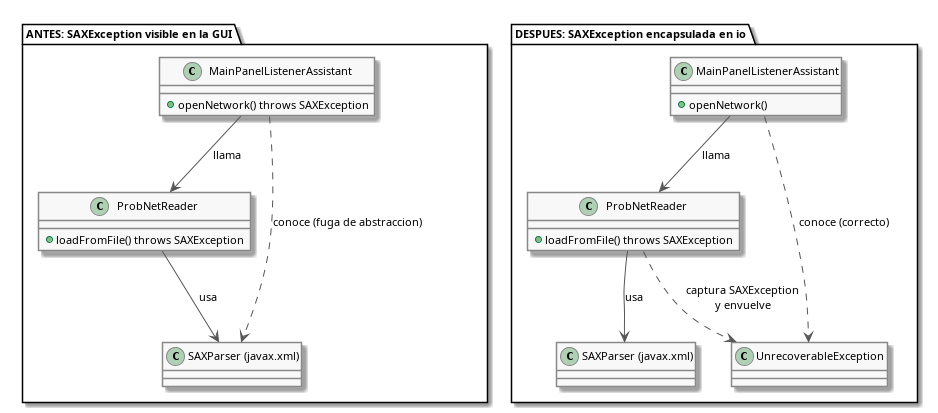
\includegraphics[width=\linewidth]{sax_before_after.png}
\caption{Fuga de \texttt{SAXException} antes (izquierda) y después (derecha) del cambio}
\label{fig:sax-before-after}
\end{figure}

\subsection{Punto 13 — Jerarquía sellada de \texttt{NonProjectablePotentialException}}

Se convirtió \texttt{NonProjectablePotentialException} en una clase sellada con
ocho subtipos internos (véase diagrama~\ref{fig:nonprojectable}):

\begin{lstlisting}[caption={Extracto de la jerarquía sellada}]
public abstract sealed class NonProjectablePotentialException
        extends OpenMarkovRuntimeException {

    public static final class SuperValueMustBeSumOrProduct
            extends NonProjectablePotentialException { ... }

    public static final class PotentialCannotBeConvertedToATable
            extends NonProjectablePotentialException { ... }

    public static final class MissingVariableInEvidence
            extends NonProjectablePotentialException { ... }
    // ... cinco tipos mas
}
\end{lstlisting}

Los beneficios concretos son:

\begin{itemize}
  \item El compilador puede comprobar la exhaustividad de los \texttt{switch}
    sobre esta excepción.
  \item Los ocho casos anteriormente informales quedan documentados con nombre
    propio y campos tipados.
  \item Es imposible añadir un nuevo subtipo «accidentalmente» desde otro módulo.
\end{itemize}

Adicionalmente se eliminaron varias clases auxiliares redundantes relacionadas
con la escritura de ficheros (\texttt{WriterException} y similares), cuya
funcionalidad quedaba ya cubierta por la jerarquía de \texttt{IOException}.

\begin{figure}[H]
\centering
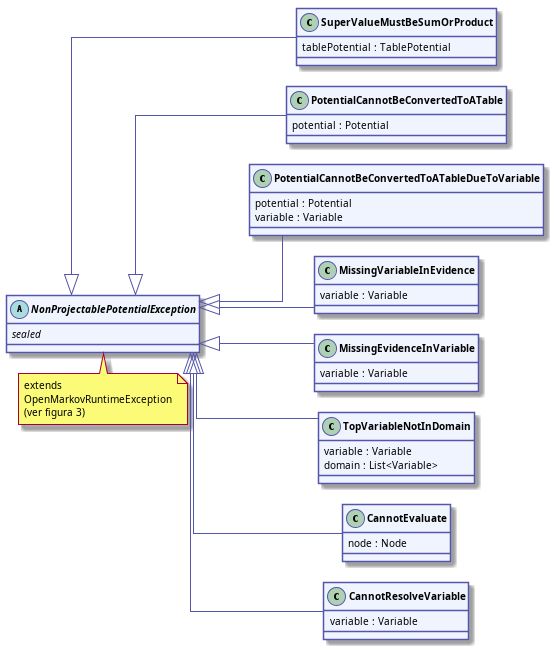
\includegraphics[width=0.6\linewidth]{nonprojectable_hierarchy.png}
\caption{Jerarquía sellada de \texttt{NonProjectablePotentialException}}
\label{fig:nonprojectable}
\end{figure}

\subsection{Punto 14 — Patrón \texttt{UIAction} en la GUI}

Se introdujo la interfaz funcional \texttt{UIAction} y el método auxiliar
\texttt{executeUIAction} en \texttt{MainPanelListenerAssistant}:

\begin{lstlisting}[caption={Interfaz funcional UIAction}]
@FunctionalInterface
private interface UIAction {
    void execute() throws Exception;
}

private void executeUIAction(UIAction action) {
    try {
        action.execute();
    } catch (RuntimeException ex) {
        throw ex;               // deja pasar unchecked sin envolver
    } catch (Exception ex) {
        throw new UnrecoverableException(ex);
    }
}
\end{lstlisting}

Los 34 bloques \texttt{try/catch} repetitivos se reemplazaron por llamadas de
una sola línea:

\begin{lstlisting}[caption={Ejemplo de uso con expresión lambda}]
case ActionCommands.OPEN_NETWORK ->
    executeUIAction(() -> openNetwork());

case ActionCommands.SAVE_NETWORK ->
    executeUIAction(() -> saveNetwork());
\end{lstlisting}

Para casos que requerían varias instrucciones se usaron lambdas de bloque:

\begin{lstlisting}[caption={Lambda de bloque para acciones con varias instrucciones}]
case ActionCommands.COMPILE_NETWORK -> executeUIAction(() -> {
    compileNetwork();
    updateMenus();
});
\end{lstlisting}

Se dejaron intencionadamente fuera del patrón dos casos:

\begin{itemize}
  \item \texttt{CHANGE\_WORKING\_MODE}: tiene lógica de recuperación propia
    (mostrar diálogo de confirmación si hay cambios sin guardar).
  \item \texttt{COST\_EFFECTIVENESS\_DETERMINISTIC}: lanza
    \texttt{UnreachableException}, no una excepción comprobada.
\end{itemize}

\subsection{Fase 3 — Clase base \texttt{OpenMarkovRuntimeException}}

Se creó una clase abstracta común para las cinco excepciones de dominio:

\begin{lstlisting}[caption={OpenMarkovRuntimeException}]
package org.openmarkov.core.exception;

public abstract class OpenMarkovRuntimeException extends RuntimeException {
    protected OpenMarkovRuntimeException() {}
    protected OpenMarkovRuntimeException(Throwable cause) { super(cause); }
}
\end{lstlisting}

Esto permite capturar en un único \texttt{catch} cualquier excepción de dominio
de OpenMarkov cuando se necesite un tratamiento uniforme, sin capturar
accidentalmente \texttt{NullPointerException} u otras excepciones del sistema.

El diagrama~\ref{fig:runtime-hierarchy} muestra la jerarquía completa.

\begin{figure}[H]
\centering
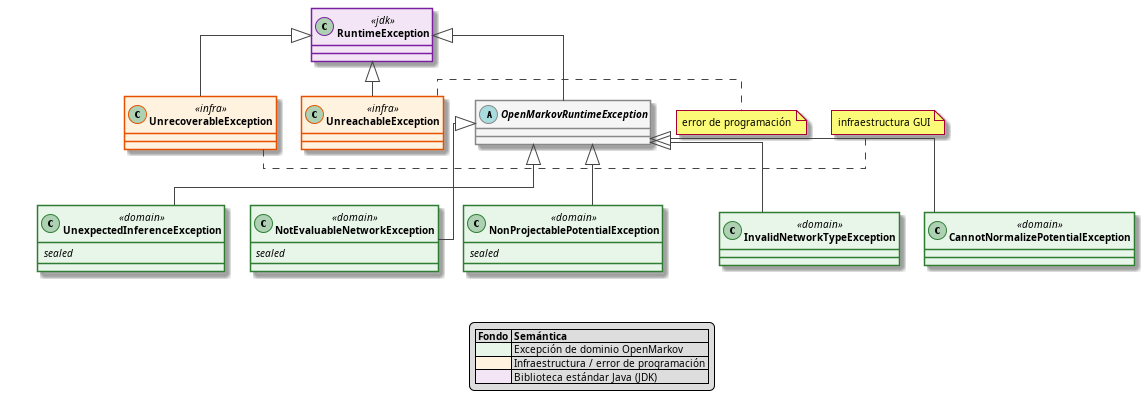
\includegraphics[width=0.85\linewidth]{runtime_hierarchy.png}
\caption{Jerarquía de excepciones de dominio bajo \texttt{OpenMarkovRuntimeException}}
\label{fig:runtime-hierarchy}
\end{figure}

\subsection{Punto 15 — Navegación de casos de evidencia}

Se eliminaron \texttt{ThereIsNoPreviousEvidenceCaseException} y
\texttt{ThereIsNoNextEvidenceCaseException}. Los bloques que las lanzaban se
sustituyeron por \texttt{UnreachableException}:

\begin{lstlisting}[caption={Guarda en goToPreviousEvidenceCase tras la refactorización}]
if (!(this.currentCase > 0)) {
    throw new UnreachableException(new IllegalStateException(
        "Go-to-previous button should have been disabled " +
        "when at first evidence case"));
}
\end{lstlisting}

La justificación es que \texttt{updateOptionsEvidenceCasesNavigation()} se llama
en todos los puntos de entrada que pueden cambiar el estado (cambio de modo de
trabajo, cada operación de navegación, cambio de opciones de propagación),
garantizando que los botones estén siempre desactivados cuando el índice está en
los extremos. La excepción original era, por tanto, código muerto.

\texttt{UnreachableException} comunica explícitamente a los futuros
mantenedores que esta rama es imposible bajo las invariantes actuales, a
diferencia de un \texttt{// never happens} en un comentario que puede quedar
desfasado.

% ─────────────────────────────────────────────────────────────────────────────
\subsection{Módulo \texttt{stochasticPropagationOutput} — Eliminación de excepciones
ya no comprobadas}
\label{sec:stochastic}

El módulo \texttt{org.openmarkov.stochasticPropagationOutput} proporciona un
diálogo secundario (\texttt{StochasticPropagationOutputFrame}) para visualizar
los resultados de la propagación estocástica. Este diálogo también invoca el
motor de inferencia y, por tanto, estaba afectado por las excepciones de dominio
convertidas en la Fase~1.

El método privado \texttt{onActionRequest()} contenía antes de la refactorización
la siguiente firma:

\begin{lstlisting}[caption={Firma antes en StochasticPropagationOutputFrame}]
private void onActionRequest()
        throws NonProjectablePotentialException,
               IncompatibleEvidenceException,
               NotEvaluableNetworkException.NotApplicableNetwork,
               NotEvaluableNetworkException.UnsatisfiedConstraints,
               ConstraintViolatedException { ... }
\end{lstlisting}

Dado que \texttt{NonProjectablePotentialException} y
\texttt{NotEvaluableNetworkException} (incluidos sus subtipos sellados) son
ahora no comprobadas, el compilador ya no exige declararlas. La cláusula
\texttt{throws} se redujo a las dos excepciones que permanecen como comprobadas:

\begin{lstlisting}[caption={Firma después en StochasticPropagationOutputFrame}]
private void onActionRequest()
        throws IncompatibleEvidenceException,
               ConstraintViolatedException { ... }
\end{lstlisting}

El bloque \texttt{catch} en \texttt{actionPerformed()} no se modificó: sigue
capturando toda excepción de dominio que alcance el \textit{event dispatch
thread} de Swing y la envuelve en \texttt{UnrecoverableException}, de forma
consistente con el patrón del Punto~14.

Este cambio es una consecuencia directa de la Fase~1: una vez que las
excepciones de dominio se vuelven no comprobadas, el compilador se encarga
automáticamente de señalar las declaraciones \texttt{throws} redundantes en
todos los módulos que las usaban.

% ─────────────────────────────────────────────────────────────────────────────
\subsection{Módulo \texttt{inference} — Modernización de \texttt{ClusterOfVariables}}
\label{sec:inference-cleanup}

La clase \texttt{ClusterOfVariables} es la clase abstracta base de los nodos de
clúster en el algoritmo de propagación de Hugin, que forma parte del módulo
\texttt{org.openmarkov.inference}. Como parte de la misma oleada de limpieza,
se aplicaron tres mejoras a esta clase:

\subsubsection*{Eliminación de importación no utilizada}

La clase importaba \texttt{NotSupportedOperationException} sin referenciarla en
ningún método. La importación fue fruto de una refactorización anterior que
movió el código que la necesitaba. Se eliminó.

\subsubsection*{Operador diamante en instancias de \texttt{ArrayList}}

Java 7 introdujo el operador diamante (\texttt{<>}) para evitar repetir el
parámetro de tipo al instanciar genéricos. \texttt{ClusterOfVariables} contenía
siete instanciaciones del estilo:

\begin{lstlisting}[caption={Antes: parámetro de tipo explícito}]
priorPotentials     = new ArrayList<TablePotential>();
evidencePotentials  = new ArrayList<TablePotential>();
separatorVariables  = new ArrayList<Variable>();
List<TablePotential> potentials = new ArrayList<TablePotential>();
List<ClusterOfVariables> otherChildren =
    new ArrayList<ClusterOfVariables>(children);
\end{lstlisting}

\begin{lstlisting}[caption={Después: operador diamante}]
priorPotentials     = new ArrayList<>();
evidencePotentials  = new ArrayList<>();
separatorVariables  = new ArrayList<>();
List<TablePotential> potentials = new ArrayList<>();
List<ClusterOfVariables> otherChildren = new ArrayList<>(children);
\end{lstlisting}

El tipo ya se declara en la variable de la izquierda; repetirlo en el
constructor es redundante y dificulta la lectura cuando los nombres de tipo
son largos.

\subsubsection*{Encadenamiento de \texttt{StringBuilder.append()} en \texttt{toString()}}

El método \texttt{toString()} de \texttt{ClusterOfVariables} construía
cadenas de texto concatenando literales con el operador \texttt{+}:

\begin{lstlisting}[caption={Antes: concatenación con +}]
out.append(((separatorVariables.size() == 1)
    ? "Separator" : "Separators") + ": {");

out.append("Prior potentials (" + priorPotentials.size() + "): ");
\end{lstlisting}

\begin{lstlisting}[caption={Después: encadenamiento de append}]
out.append((separatorVariables.size() == 1)
    ? "Separator" : "Separators").append(": {");

out.append("Prior potentials (").append(priorPotentials.size()).append("): ");
\end{lstlisting}

Aunque la diferencia de rendimiento es nula en métodos de diagnóstico,
el encadenamiento resulta más legible cuando el \texttt{StringBuilder} ya está
presente, y es el estilo preferido en el resto de la clase.

% ─────────────────────────────────────────────────────────────────────────────
\section{Decisiones de diseño}
\label{sec:decisiones}

\subsection{Preservación de nombres existentes}

Una versión anterior del plan proponía renombrar varias excepciones para
encajarlas en una nueva taxonomía (p.\,ej.,
\texttt{NonProjectablePotentialException} $\to$
\texttt{PotentialComputationException}). Se descartó esta opción porque:

\begin{itemize}
  \item Los nombres originales (\texttt{NonProjectablePotentialException},
    \texttt{CannotNormalizePotentialException}, \texttt{InvalidNetworkTypeException},
    \texttt{DoEditException}) son vocabulario establecido entre los programadores
    de OpenMarkov y tienen significado semántico preciso en el dominio de las
    redes probabilísticas.
  \item El cambio de nombre habría requerido actualizar cientos de ficheros en
    todos los módulos, introduciendo ruido en el historial de control de
    versiones sin beneficio funcional.
  \item La taxonomía se puede expresar igualmente bien con herencia, sin imponer
    renombrados.
\end{itemize}

\subsection{\texttt{DoEditException} permanece como excepción comprobada}

\texttt{DoEditException} no se convirtió a no comprobada. Esta excepción señaliza
un fallo en la ejecución de una edición de la red (operación de
\textit{undo/redo}) y tiene puntos de captura específicos con lógica de
tratamiento. Convertirla requeriría revisar esa lógica, con riesgo de introducir
regresiones en el sistema de deshacer/rehacer. El consenso fue que el coste
superaba el beneficio en este caso.

\subsection{Exclusión de \texttt{UnreachableException} y \texttt{UnrecoverableException} de la jerarquía de dominio}

Estas dos excepciones tienen naturaleza distinta a las cinco de dominio:

\begin{description}[leftmargin=2em]
  \item[\texttt{UnreachableException}] Señaliza código que \emph{por diseño}
    nunca debería ejecutarse (equivalente a \texttt{assert false}). No es un
    error de dominio sino un fallo de programación.
  \item[\texttt{UnrecoverableException}] Es infraestructura de la GUI: envuelve
    cualquier excepción que alcanza el \textit{event dispatch thread} de Swing
    sin haber sido tratada. Su alcance es transversal, no específico del dominio
    de redes probabilísticas.
\end{description}

Incluirlas en \texttt{OpenMarkovRuntimeException} habría mezclado semánticas muy
diferentes, dificultando bloques \texttt{catch} que intenten tratar
específicamente errores de dominio sin capturar errores de programación.

\subsection{Excepciones que permanecen comprobadas en \\\texttt{stochasticPropagationOutput}}

En el módulo \texttt{stochasticPropagationOutput}, \texttt{IncompatibleEvidenceException}
y \texttt{ConstraintViolatedException} se mantuvieron en la cláusula
\texttt{throws} de \texttt{onActionRequest()} porque siguen siendo excepciones
comprobadas: representan condiciones de error que el llamador puede
razonablemente anticipar y manejar (evidencia inconsistente con la red, o
restricción de modelo violada). Su naturaleza comprobada es, por tanto,
correcta e intencionada.

\subsection{Alcance de la modernización en \texttt{ClusterOfVariables}}

Los cambios en \texttt{ClusterOfVariables} (operador diamante, importación
eliminada, encadenamiento de \texttt{append}) no afectan al comportamiento
observable del algoritmo. Se incluyeron en la misma oleada de limpieza porque:

\begin{itemize}
  \item El fichero fue identificado al revisar los módulos que importaban las
    excepciones convertidas.
  \item La presencia de código de estilo más antiguo en un fichero muy estable
    hacía que la revisión resultara más costosa de lo necesario.
  \item El riesgo de regresión es mínimo: las modificaciones son puramente
    sintácticas y la semántica del algoritmo no cambia.
\end{itemize}

% ─────────────────────────────────────────────────────────────────────────────
\section{Impacto cuantitativo global}
\label{sec:impacto}

\begin{table}[H]
\centering
\begin{tabularx}{\textwidth}{p{6.5cm}rX}
\toprule
Cambio & Ficheros afectados & Elementos eliminados/añadidos \\
\midrule
Conversión checked $\to$ unchecked (5 excepciones) & 53 & $-$40 cláusulas \texttt{throws} \\
Encapsulación de \texttt{SAXException} &  1 & $-$1 \texttt{throws SAXException} en GUI \\
Jerarquía sellada \texttt{NonProjectablePotentialException} & 1 & $+$8 subtipos tipados \\
Patrón \texttt{UIAction} &  1 & $-$34 bloques \texttt{try/catch} repetitivos \\
\texttt{OpenMarkovRuntimeException} &  6 & $+$1 clase base; $+$5 relaciones de herencia \\
Eliminación excepciones de navegación &  3 & $-$2 clases de excepción \\
\texttt{StochasticPropagationOutputFrame} &  1 & $-$2 tipos de la cláusula \texttt{throws} \\
\texttt{ClusterOfVariables} (modernización) &  1 & $-$1 importación; $-$7 tipos genéricos explícitos \\
\midrule
\textbf{Total} & \textbf{67} & net $-$79 elementos \\
\bottomrule
\end{tabularx}
\caption{Resumen cuantitativo de la refactorización}
\label{tab:impacto}
\end{table}

% ─────────────────────────────────────────────────────────────────────────────
\section{Conclusiones}
\label{sec:conclusiones}

La refactorización elimina aproximadamente 79 elementos de código redundante o
problemático, distribuidos en 67 ficheros a lo largo de seis módulos. El impacto
neto es positivo en múltiples dimensiones:

\begin{itemize}
  \item \textbf{Legibilidad}: los métodos expresan su lógica sin distracciones
    de manejo de errores que no aportan información.
  \item \textbf{Mantenibilidad}: añadir una nueva acción en \texttt{actionPerformed}
    ya no requiere recordar el patrón \texttt{try/catch} repetitivo.
  \item \textbf{Seguridad estática}: la jerarquía sellada de
    \texttt{NonProjectablePotentialException} permite que el compilador detecte
    bloques \texttt{switch} no exhaustivos.
  \item \textbf{Separación de capas}: la GUI ya no conoce detalles de
    implementación de la capa de E/S (\texttt{SAXException}).
  \item \textbf{Expresividad de intención}: \texttt{UnreachableException}
    documenta en el código mismo que una rama es imposible según las invariantes
    del sistema, de forma verificable y no perecedera como un comentario.
  \item \textbf{Propagación sistemática}: la conversión de excepciones de
    dominio a no comprobadas se aplicó de forma consistente en todos los módulos
    afectados (\texttt{gui}, \texttt{inference}, \texttt{learning.algorithm},
    \texttt{stochasticPropagationOutput}), evitando que quedaran restos del
    sistema antiguo en capas periféricas.
\end{itemize}

Todos los tests existentes pasan después de los cambios, lo que proporciona
confianza en que no se han introducido regresiones en el comportamiento
observable.

\end{document}
